\section{Desarrollo Teórico}\label{sec:teoria}
\subsection{Modelo atómico de tres niveles}
%region
Consideremos un sistema atómico de tres niveles en configuración $\Lambda$ acoplado a dos haces de luz coherente como se muestra en la figura \ref{fig:eit_diagram}. El sistema consiste en un estado fundamental $\ket{1}$ de energía $E_1 = \hbar \omega_1$, un estado metaestable $\ket{2}$ con energía $E_2 = \hbar \omega_2$ de mayor energía ($\omega_1 < \omega_2$) y un estado excitado común $\ket{3}$ con energía $E_3 = \hbar \omega_3$. Veamos que la transición hiperfina $\ket{1} \to \ket{2}$ está prohibida debido a las reglas de selección del dipolo eléctrico ($\mu_{12}=0$). El sistema atómico interactúa con un haz de prueba (\textit{probe}) de frecuencia $\omega_p$ que acopla la transición $\ket{1} \to \ket{3}$ con frecuencia Rabi $\Omega_p$ y un haz de control (\textit{control}) de frecuencia $\omega_c$ que acopla la transición $\ket{2} \to \ket{3}$ con frecuencia Rabi $\Omega_c$ \cite{footAtomicPhysics2005, alzettaExperimentalMethodObservation1976}.

\begin{figure}[ht]
    \centering
    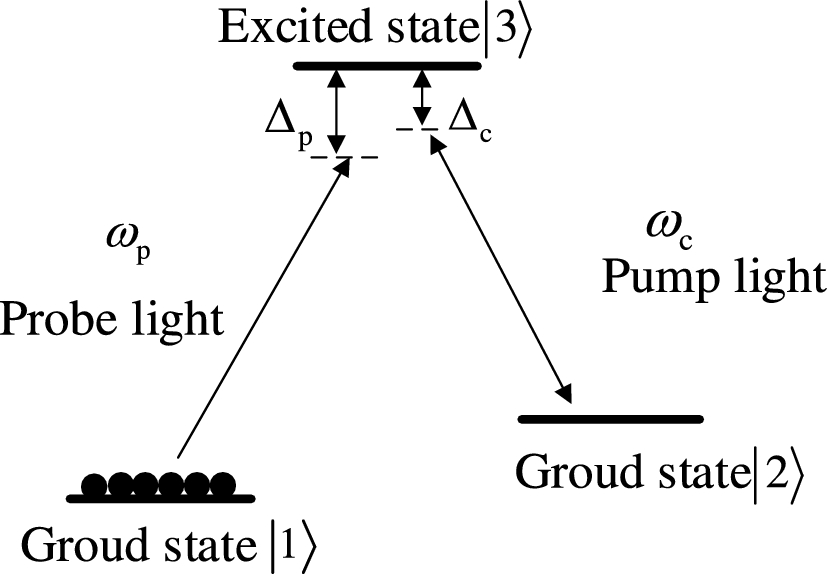
\includegraphics[height = 6cm]{figures/EIT_diagram.png}
    \captionof{figure}{Diagrama de sistema atómico de tres niveles en configuración $\Lambda$. El sistema además interactúa con un haz de prueba y un haz de control.}
    \label{fig:eit_diagram}
\end{figure}

Por simplicidad definamos las desintonías entre los haces de luz y las trancisiones atómicas como \cite{scullyQuantumOptics1997a,footAtomicPhysics2005},
\begin{equation}
\begin{split}
    \Delta_p &= \omega_p -\omega_{31} = \omega_p - (\omega_3 - \omega_1), \\
    \Delta_c &= \omega_c - \omega_{32} = \omega_c - (\omega_3- \omega_2), \\
    \delta &= \Delta_p - \Delta_c = (\omega_p- \omega_c) - \omega_{21} = (\omega_p- \omega_c) - (\omega_2 - \omega_1).
\end{split}
\end{equation}
%endregion

\subsubsection*{Hamiltoniano del sistema}
El hamiltoniano del sistema estará dado por la suma del hamiltoniano atómico libre $\hat{H}^{(0)}$ y el término de interacción con el campo electromagnético $\hat{H}^{(1)}(t)$ \cite{gerryIntroductoryQuantumOpticsa, fleischhauerElectromagneticallyInducedTransparency2005},
\begin{equation}
\hat{H} = \hat{H}^{(0)} + \hat{H}^{(1)}(t)
\end{equation}
Para el \textbf{hamiltoniano atómico libre} $\hat{H}^{(0)}$ tenemos que las eigenfunciones y eigenenergías estarán dados por $\hat{H}^{(0)} \ket{i} = E_i \ket{i}$ donde $\ket{i}$ son los niveles de energía en los que el sistema puede encontrarse e $i = \{1, 2, 3\}$ representan los estados respectivos.
\begin{equation}
\hat{H}^{(0)} = \sum_{i=1}^{3} E_i \ket{i}\bra{i} = \hbar \omega_1 \ket{1}\bra{1} + \hbar \omega_2 \ket{2}\bra{2} + \hbar \omega_3 \ket{3}\bra{3}
\end{equation}
Por ortonormalidad de la base $\{\ket{i}\}$ sabemos que $\hat{H}^{(0)}$ es diagonal ($\bra{i} \hat{H}^{(0)} \ket{j} = E_i \delta_{ij}$). Fijando la energía del estado fundamental como referencia ($E_1 = 0$), el hamiltoniano queda expresado como una matriz diagonal de la forma,
\begin{equation}
\hat{H}^{(0)} = \begin{pmatrix}
E_1 &  0 & 0 \\
0 & E_2 & 0 \\
0 & 0 & E_3
\end{pmatrix} = \hbar \begin{pmatrix}
    0 & 0 & 0 \\
    0 & \omega_{21} & 0 \\
    0 &  0 & \omega_{31}
\end{pmatrix}
\end{equation}

Por otro lado, para el \textbf{hamiltoniano de interacción} $\hat{H}^{(1)}(t)$, bajo la aproximación dipolar eléctrica \cite{robertw.boydNonlinearOptics,steckQuantumAtomOptics2007} tenemos que la interacción entre el sistema atómica y el campo electromagnético estará dada por $\hat{H}^{(1)}(t) = - \hat{\vec{\mu}} \cdot \vec{E}(t)$ donde $\hat{\vec{\mu}}$ es el operador de momento dipolar eléctrico y $\vec{E}(t)$ es el campo eléctrico de interacción.

Para el sistema de tres niveles en configuración $\Lambda$ debido a las reglas de selección de paridad, los elementos diagonales se anulan ($\vec{\mu}_{ii} =0$) y la transición $\ket{1} \to \ket{2}$ está prohibida ($\vec{\mu}_{12} = 0$). Por lo que el operador de momento dipolar queda descrito como, 
\begin{equation}
\hat{\vec{\mu}}= \vec{\mu}_{31} \ket{3}\bra{1} +  \vec{\mu}_{13} \ket{1}\bra{3} + \vec{\mu}_{32} \ket{3}\bra{2} + \vec{\mu}_{23} \ket{2}\bra{3}
\end{equation}
O bien en notación matricial,
\begin{equation}
    \hat{\vec{\mu}} = \begin{pmatrix}
        0 & 0 & \vec{\mu}_{31}^* \\ 
        0 & 0 & \vec{\mu}_{32}^*\\
        \vec{\mu}_{31} & \vec{\mu}_{32} & 0
    \end{pmatrix}
\end{equation}
En este caso, asumimos que los estados atómicos tienen una paridad definida y que sus funciones de onda son reales, de modo que el operador de momento dipolar es hermítico ($\vec{\mu}_{ij} = \vec{\mu}_{ji}^*$).

Ahora, el campo eléctrico total $\vec{E}(t)$ está dado por la superposición clásica de los dos haces de luz coherentes $\vec{E}(t) = \vec{E}_p(t) + \vec{E}_c(t)$. En términos de la amplitud compleja de los campos,
\begin{equation}
    \vec{E}(t) = \frac{1}{2}\vec{\varepsilon}_p e^{-i\omega_p t} + \frac{1}{2}\vec{\varepsilon}_c e^{-i\omega_c t} + \text{c.c.}
\end{equation}
Evaluando en el hamiltoniano de interacción obtenemos,
\begin{equation}
\hat{H}^{(1)}(t) = - \left[ \vec{\mu}_{31} (\ket{3}\bra{1} + \ket{1}\bra{3}) + \vec{\mu}_{32} (\ket{3}\bra{2} + \ket{2}\bra{3}) \right] \cdot \frac{1}{2} \left[ \vec{\varepsilon}_p e^{-i\omega_p t} + \vec{\varepsilon}_c e^{-i\omega_c t} + \text{c.c.} \right]
\end{equation}
De forma que el hamiltoniano total del sistema queda expresado como,
\begin{equation}
    \hat{H}(t) = \begin{pmatrix}
    \hbar \omega_1 & 0 & - \frac{1}{2}\vec{\mu}_{13} \cdot \vec{E}(t) \\
    0 & \hbar \omega_2 & - \frac{1}{2}\vec{\mu}_{23} \cdot \vec{E}(t) \\
    -\frac{1}{2}\vec{\mu}_{13} \cdot \vec{E}(t) & -\frac{1}{2}\vec{\mu}_{23} \cdot \vec{E}(t) & \hbar \omega_3
    \end{pmatrix}
\end{equation}

\subsubsection*{Marco de Interacción}
Resulta conveniente movernos al marco de interacción, donde el hamiltoniano toma una forma más simple. Definimos el operador de evolución temporal $\hat{U}_0(t)$ y su operador adjunto  $\hat{U}_0^{\dagger}(t)$,
\begin{equation}
\hat{U}_0(t) = e^{-i \hat{H}^{(0)}t} = \begin{pmatrix}
    1 & 0 & 0 \\
    0 & e^{-i\omega_{21} t} & 0 \\
    0 & 0 & e^{-i\omega_{31} t}
\end{pmatrix}, \quad  \hat{U}_0(t)^{\dagger} = \begin{pmatrix}
    1 & 0 & 0 \\
    0 & e^{i\omega_{21} t} & 0 \\
    0 & 0 & e^{i\omega_{31} t}
\end{pmatrix}
\end{equation}
El hamiltoniano en este nuevo cuadro se obtiene a partir de la regla de transformación,
\begin{equation}
\hat{H}'(t) = \hat{U} \hat{H}(t) \hat{U}^{\dagger} + i \hbar \left(\pdv{\hat{U}(t)}{t}\right) \hat{U}^{\dagger}(t)
\end{equation} 
obtenemos la matriz del hamiltoniano en el marco de interacción. Dado que,
\begin{equation}
    i \hbar \pdv{\hat{U}(t)}{t} \hat{U}^{\dagger}(t) = i \hbar \left(\frac{i}{\hbar} \hat{H}^{(0)} \hat{U}(t)\right)  \hat{U}^{\dagger}(t) = - \hat{H}^{(0)}
\end{equation}
Sustituyendo al hamiltoniano $\hat{H}(t) = \hat{H}^{(0)} + \hat{H}^{(1)}(t)$ en la ecuación obtenemos que el hamitloniano en el marco de interacción queda dado como,
\begin{equation}
\begin{split}
\hat{H}_{int}(t) &= \hat{U} (\hat{H}^{(0)} + \hat{H}^{(1)}(t)) \hat{U}^{\dagger} + i \hbar \pdv{\hat{U}(t)}{t} \hat{U}^{\dagger}(t) \\
&= \hat{U} \hat{H}^{(0)} \hat{U}^{\dagger} + \hat{U} \hat{H}^{(1)}(t) \hat{U}^{\dagger} - \hat{H}^{(0)} \\
&= \hat{H}^{(0)} - \hat{H}^{(0)} + \hat{U} \hat{H}^{(1)}(t) \hat{U}^{\dagger} = \hat{U} \hat{H}^{(1)}(t) \hat{U}^{\dagger}
\end{split}
\end{equation}
Realizando la operación matricial obtenemos el hamiltoniano en el marco de interacción,
\begin{equation}
\hat{H}_{int}(t) = \hat{U} \hat{H}^{(1)}(t) \hat{U}^{\dagger} = -\begin{pmatrix}
0 & 0 & \left( \vec{\mu_{31}^*} \cdot \vec{E}(t)\right) e^{-i\omega_{31}t}\\
0 & 0 & \left( \vec{\mu_{32}^*} \cdot \vec{E}(t)\right) e^{-i\omega_{32}t}\\
\left( \vec{\mu_{31}} \cdot \vec{E}(t)\right) e^{i\omega_{31}t} & \left( \vec{\mu_{32}} \cdot \vec{E}(t)\right) e^{i\omega_{32}t} & 0 
\end{pmatrix}
\end{equation}

\subsubsection*{Aproximación de Onda Rotante}
Sustituyendo el campo eléctrico total $\vec{E}(t) = \vec{\varepsilon}_p e^{-i\omega_p t} + \vec{\varepsilon}_p^* e^{i\omega_p t} + \vec{\varepsilon}_c e^{-i\omega_c t} + \vec{\varepsilon}_c^* e^{i\omega_c t}$ para cada elemento distinto de cero obtenemos,
\begin{equation*}
\begin{split}
\left[ \hat{H}_{int}(t)\right]_{13} &= - \left( \vec{\mu_{31}^*} \cdot \vec{E}(t)\right) e^{-i\omega_{31}t} \\ 
&= - \frac{1}{2} \left[ (\vec{\mu_{31}^*} \cdot \vec{\varepsilon}_p)e^{-i(\omega_p + \omega_{31}) t} + (\vec{\mu_{31}^*} \cdot \vec{\varepsilon}_p^*)  e^{i(\omega_p - \omega_{31}) t} + (\vec{\mu_{31}^*} \cdot \vec{\varepsilon}_c) e^{-i(\omega_c + \omega_{31}) t} + (\vec{\mu_{31}^*} \cdot \vec{\varepsilon}_c^*)e^{i(\omega_c - \omega_{31}) t}
\right]
\end{split}
\end{equation*}

\begin{equation*}
\begin{split}
\left[ \hat{H}_{int}(t)\right]_{31} &= - \left( \vec{\mu_{31}} \cdot \vec{E}(t)\right) e^{i\omega_{31}t} \\ 
&= - \frac{1}{2} \left[ (\vec{\mu_{31}} \cdot \vec{\varepsilon}_p)e^{-i(\omega_p - \omega_{31}) t} + (\vec{\mu_{31}} \cdot \vec{\varepsilon}_p^*)  e^{i(\omega_p + \omega_{31}) t} + (\vec{\mu_{31}} \cdot \vec{\varepsilon}_c) e^{-i(\omega_c - \omega_{31}) t} + (\vec{\mu_{31}} \cdot \vec{\varepsilon}_c^*)e^{i(\omega_c + \omega_{31}) t}
\right]
\end{split}
\end{equation*}

\begin{equation*}
\begin{split}
\left[ \hat{H}_{int}(t)\right]_{23} &= - \left( \vec{\mu_{32}^*} \cdot \vec{E}(t)\right) e^{-i\omega_{32}t} \\ 
&= - \frac{1}{2} \left[ (\vec{\mu_{32}^*} \cdot \vec{\varepsilon}_p)e^{-i(\omega_p + \omega_{32}) t} + (\vec{\mu_{32}^*} \cdot \vec{\varepsilon}_p^*)  e^{i(\omega_p - \omega_{32}) t} + (\vec{\mu_{32}^*} \cdot \vec{\varepsilon}_c) e^{-i(\omega_c + \omega_{32}) t} + (\vec{\mu_{32}^*} \cdot \vec{\varepsilon}_c^*)e^{i(\omega_c - \omega_{32}) t}
\right]
\end{split}
\end{equation*}

\begin{equation*}
\begin{split}
\left[ \hat{H}_{int}(t)\right]_{32} &= - \left( \vec{\mu_{32}} \cdot \vec{E}(t)\right) e^{i\omega_{32}t} \\ 
&= - \frac{1}{2} \left[ (\vec{\mu_{32}} \cdot \vec{\varepsilon}_p)e^{-i(\omega_p - \omega_{32}) t} + (\vec{\mu_{32}} \cdot \vec{\varepsilon}_p^*)  e^{i(\omega_p + \omega_{32}) t} + (\vec{\mu_{32}} \cdot \vec{\varepsilon}_c) e^{-i(\omega_c - \omega_{32}) t} + (\vec{\mu_{32}} \cdot \vec{\varepsilon}_c^*)e^{i(\omega_c + \omega_{32}) t}
\right]
\end{split}
\end{equation*}
Cerca de resonancia para ambos láseres, la frecuencia de cada haz de luz es aproximadamente igual a la frecuencia de trancisión atómica ($\omega_p \approx \omega_{31}, \omega_c \approx \omega_{32}$).

Veamos que para los elementos $(1,3)$ y $(3,1)$ de la matriz tenemo distintos elementos de exponenciales temporales que podemos separar en tres casos específicos
\begin{itemize}
    \item Los elementos $\bm{e^{\pm  i(\omega_p-\omega_{31})}}$. Como $\omega_p \approx \omega_{31}$, $\omega_p-\omega_{31}$ cercano a cero y la exponencial varía lentamente con el tiempo.
    \item Los elementos $\bm{e^{\pm  i(\omega_p+\omega_{31})}}$. Éstos oscilan cerca de $\omega_p + \omega_{31} \approx 2\omega_{31}$, que es una frecuencia muy alta comparada con la frecuencia de trancisión atómica. Por lo que estos términos varían rápidamente con el tiempo y su promedio temporal es cero. 
    \item Los elementos $\bm{e^{\pm  i(\omega_c \pm \omega_{31})}}$. Dado que el láser de control $\omega_c$ está sintonizado a la transición $\ket{2} \to \ket{3}$ y no para la transición $\ket{1} \to  \ket{3}$, éstas combinaciones se encuentra fuertemente fuera de resonancia y oscilan a frecuencias ópticas por lo que de misma forma su promedio temporal es cero.
\end{itemize}
De la misma forma para los elementos $(2,3)$ y $(3,2)$ de la matriz, los términos que varían lentamente con el tiempo son $\bm{e^{\pm  i(\omega_c-\omega_{32})}}$ y los que varían rápidamente con el tiempo son $\bm{e^{\pm  i(\omega_c+\omega_{32})}}$ y $\bm{e^{\pm  i(\omega_p \pm \omega_{32})}}$. A partir de la \textbf{aproximación de onda rotante} (RWA) podemos despreciar los terminos de oscilación rápida debido a que su promedio temporal es cero, obteniendo el hamiltoniano en el marco de interacción bajo ésta aproximación.
\begin{equation}
\begin{split}
\hat{H}_{RWA} &= -\begin{pmatrix}
0 & 0 & \frac{1}{2}(\vec{\mu}_{31}^* \cdot \vec{\varepsilon}_{p}^*) e^{-i(\omega_p - \omega_{31})t} \\
0 & 0 & \frac{1}{2}(\vec{\mu}_{32}^* \cdot \vec{\varepsilon}_{c}^*) e^{-i(\omega_c - \omega_{32})t} \\
\frac{1}{2}(\vec{\mu}_{31} \cdot \vec{\varepsilon}_{p}) e^{i(\omega_p - \omega_{31})t} & \frac{1}{2}(\vec{\mu}_{32} \cdot \vec{\varepsilon}_{c}) e^{i(\omega_c - \omega_{32})t} & 0
\end{pmatrix}\\
&= - \hbar \begin{pmatrix}
0 & 0 & \frac{\Omega_p^*}{2} e^{-i \Delta_p t} \\
0 & 0 & \frac{\Omega_c^*}{2} e^{-i \Delta_c t} \\
\frac{\Omega_p}{2} e^{i \Delta_p t} & \frac{\Omega_c}{2} e^{i \Delta_c t} & 0
\end{pmatrix}
\end{split}
\end{equation}
O bien en notación de Dirac,
\begin{equation}
\hat{H}_{RWA} = - \frac{\hbar}{2} \left( \Omega_p e^{i \Delta_p t} \ket{3}\bra{1} + \Omega_c e^{i \Delta_c t} \ket{3}\bra{2} + \text{h.c.} \right)
\end{equation}
donde hemos definido a las frecuencias de Rabi $\Omega_p = \frac{\vec{\mu}_{31} \cdot \vec{E}_p}{\hbar}$,  $\Omega_c = \frac{\vec{\mu}_{32} \cdot \vec{E}_c}{\hbar}$ y sus conjugadas complejas $\Omega_p^* = \frac{\vec{\mu}_{31}^* \cdot \vec{E}_p^*}{\hbar}$,  $\Omega_c^* = \frac{\vec{\mu}_{32}^* \cdot \vec{E}_c^*}{\hbar}$.

\subsubsection*{Marco Rotante}
Para tener un marco de referencia donde el hamiltoniano no dependa del tiempo, realizamos ahora una transformación unitaria al marco rotante. Proponemos entonces la matriz unitaria de transformación $\hat{U}(t)$ y su adjunta $\hat{U}^{\dagger}(t)$ como,
\begin{equation}
    \hat{U}(t)= \begin{pmatrix}
    1 & 0 & 0 \\
    0 & e^{-i(\Delta_p-\Delta_c) t} & 0 \\
    0 & 0 & e^{-i\Delta_p t}
    \end{pmatrix}, \quad
    \hat{U}^{\dagger}(t)= \begin{pmatrix}
    1 & 0 & 0 \\
    0 & e^{i(\Delta_p-\Delta_c) t} & 0 \\
    0 & 0 & e^{i\Delta_p t}
    \end{pmatrix}
\end{equation}
A partir de la regla de transformación $\hat{H}_{rot} = \hat{U}(t) \hat{H}_{RWA} \hat{U}^{\dagger}(t) - i \hbar \hat{U}(t) \dv{t} \hat{U}^{\dagger}(t)$ obtenemos el hamiltoniano en el marco rotante. Veamos que
\begin{equation}
\begin{split}
\hat{U}(t) \hat{H}_{RWA} \hat{U}^{\dagger}(t) &= - 
\hbar 
\begin{pmatrix}
    1 & 0 & 0 \\
    0 & e^{-i(\Delta_p-\Delta_c) t} & 0 \\
    0 & 0 & e^{-i\Delta_p t}
\end{pmatrix}
\begin{pmatrix}
0 & 0 & \frac{\Omega_p^*}{2} e^{-i \Delta_p t} \\
0 & 0 & \frac{\Omega_c^*}{2} e^{-i \Delta_c t} \\
\frac{\Omega_p}{2} e^{i \Delta_p t} & \frac{\Omega_c}{2} e^{i \Delta_c t} & 0
\end{pmatrix}
\begin{pmatrix}
    1 & 0 & 0 \\
    0 & e^{i(\Delta_p-\Delta_c) t} & 0 \\
    0 & 0 & e^{i\Delta_p t}
\end{pmatrix}\\
&= - \hbar\begin{pmatrix}
0 & 0 & \frac{\Omega_p^*}{2} e^{-i \Delta_p t}  e^{i\Delta_p t} \\
0 & 0 & \frac{\Omega_c^*}{2} e^{-i \Delta_c t} e^{-i(\Delta_p-\Delta_c) t} e^{i\Delta_p t} \\
\frac{\Omega_p}{2} e^{i \Delta_p t} e^{-i\Delta_p t} & \frac{\Omega_c}{2} e^{i \Delta_c t} e^{-i\Delta_p t} e^{i(\Delta_p-\Delta_c) t} & 0
\end{pmatrix}\\
&= - \hbar \begin{pmatrix}
0 & 0 & \frac{\Omega_p^*}{2}  \\
0 & 0 & \frac{\Omega_c^*}{2}  \\
\frac{\Omega_p}{2} & \frac{\Omega_c}{2} & 0
\end{pmatrix}
\end{split}
\end{equation}
Para la parte temporal de la transformación,
\begin{equation}
\begin{split}
    i \hbar \pdv{\hat{U}(t)}{t} \hat{U}^{\dagger}(t) &= i \hbar \begin{pmatrix}
    0 & 0 & 0 \\
    0 & -i(\Delta_p-\Delta_c)e^{-i(\Delta_p- \Delta_c)t} & 0 \\
    0 & 0 &  -i \Delta_p e^{-i \Delta_p t}
    \end{pmatrix} 
    \begin{pmatrix}
    0 & 0 & 0 \\
    0 & e^{i(\Delta_p- \Delta_c)t} & 0 \\
    0 & 0 &  e^{i \Delta_p t}
    \end{pmatrix}
    = \hbar 
    \begin{pmatrix}
    0 & 0 & 0 \\
    0 & \delta & 0 \\
    0 & 0 &  \Delta_p \\
    \end{pmatrix}
\end{split}
\end{equation}
Sustituyendo en la expresión de la transformación unitarioa depende del tiempo,
\begin{equation}
\hat{H}_{rot} = - \hbar \begin{pmatrix}
0 & 0 & \frac{\Omega_p^*}{2}  \\
0 & 0 & \frac{\Omega_c^*}{2}  \\
\frac{\Omega_p}{2} & \frac{\Omega_c}{2} & 0
\end{pmatrix} + \hbar 
\begin{pmatrix}
    0 & 0 & 0 \\
    0 & \delta & 0 \\
    0 & 0 &  \Delta_p \\
\end{pmatrix} = - \hbar \begin{pmatrix}
0 & 0 & \frac{\Omega_p^*}{2}  \\
0 & - \delta & \frac{\Omega_c^*}{2}  \\
\frac{\Omega_p}{2} & \frac{\Omega_c}{2} & - \Delta_p
\end{pmatrix}
\end{equation}
Obtenemos entonces el hamiltoniano en el marco rotante \cite{robertw.boydNonlinearOptics,scullyQuantumOptics1997a}, 
\begin{equation}
\boxed{
\hat{H}_{rot} = - \hbar \begin{pmatrix}
0 & 0 & \frac{\Omega_p^*}{2}  \\
0 & - \delta & \frac{\Omega_c^*}{2}  \\
\frac{\Omega_p}{2} & \frac{\Omega_c}{2} & - \Delta_p
\end{pmatrix}= - \frac{\hbar}{2} \begin{pmatrix}
    0 & 0 & \Omega_p^* \\
    0 & - 2 \delta & \Omega_c^* \\
    \Omega_p & \Omega_c & - 2 \Delta_p
\end{pmatrix}.
}    
\end{equation}
O bien en notación de Dirac,
\begin{equation*}
\hat{H}_{rot} = - \hbar \Delta_p \ket{3}\bra{3} - \hbar \delta \ket{2}\bra{2} - \frac{\hbar}{2} \left( \Omega_p \ket{3}\bra{1} + \Omega_c \ket{3}\bra{2} + \text{h.c.} \right)
\end{equation*}

\subsubsection*{Ecuación de Liouville-von Neumann}
Debido a que el sistema está compuesto por un estado mezclado $\ket{\Phi}$ resulta complicado expresar el estado completo del sistema a partir de los estados individuales y la ecuación de Schrödinger. En este caso, resulta conveniente utilizar el formalismo de la matriz de densidad $\rho$.
\begin{equation}
    \rho = \sum_s p(s) \ket{\Psi_s}\bra{\Psi_s}
\end{equation}
donde $p(s)$ representa la probabilidad de hallar un átomo del ensamble en el estado $\ket{\Psi_s}$, siempre con la condición de normalización $\text{Tr}(\rho) = 1$. Para un sistema de $n$ niveles, la matriz densidad es una matriz $n \times n$. Aquí, $\rho_{ii}$ es la población del nivel $i$ que representa los átomos en el estado $\ket{i}$ y los elementos fuera de la diagonal $\rho_{ij}$ con $i \neq j$ son las coherencias entre los niveles $i$ y $j$ que representan los átomos en la trancisión $\ket{i} \to \ket{j}$. 

Ahora, cada estado puro $\ket{\Psi_s(t)}$ obedece la ecuación de Schrödinger dependiente del tiempo,
\begin{equation}
    i \hbar \pdv{}{t} \ket{\Psi_s(t)} = \hat{H} \ket{\Psi_s(t)}
\end{equation}
Conjugando la ecuación y recordando que el hamiltoniano es hermítico ($\hat{H}^{\dagger} = \hat{H}$) obtenemos la ecuación de evolución temporal para $\bra{\Psi_s(t)}$,
\begin{equation}
    -i \hbar \pdv{}{t} \bra{\Psi_s(t)} =  \bra{\Psi_s(t)} \hat{H}
\end{equation}
Derivamos a la matriz densidad $\rho$ respecto al tiempo,
\begin{equation}
    \pdv{\rho}{t} = \pdv{}{t}\left( \sum_s p(s) \ket{\Psi_s}\bra{\Psi_s} \right) = \sum_s p(s) \pdv{}{t} \left( \ket{\Psi_s}\bra{\Psi_s} \right)
\end{equation}
Aplicamos la regla del producto a la derivada con respecto al tiempo y sustituimos las ecuaciones de evolución temporal ya conocidas,
\begin{equation}
\begin{split}
    \pdv{\rho}{t} &= \sum_s p(s) \left[ (\pdv{}{t} \ket{\Psi_s(t)})\bra{\Psi_s(t)} + \ket{\Psi_s(t)}(\pdv{}{t} \bra{\Psi_s(t)})\right]\\
    &= \sum_s p(s) \left[ (-\frac{i}{\hbar} \hat{H}\ket{\Psi_s(t)})\bra{\Psi_s(t)} +  \ket{\Psi_s(t)} (\frac{i}{\hbar} \bra{\Psi_s(t)} \hat{H} )\right]\\
    &= -\frac{i}{\hbar} \sum_s p(s) \left[\hat{H}\ket{\Psi_s(t)}\bra{\Psi_s(t)} - \ket{\Psi_s(t)} \bra{\Psi_s(t)}\hat{H} \right] 
\end{split}
\end{equation}
Dado que el hamiltoniano $\hat{H}$ es un operador lineal y $p_k$ son constantes distribuimos la suma y sustituimos con la definición de matriz densidad,
\begin{equation}
    \pdv{\rho}{t} = -\frac{i}{\hbar} \left[\hat{H} \left(\sum_s p(s) \ket{\Psi_s(t)}\bra{\Psi_s(t)} \right) - \left( \sum_s p(s) \ket{\Psi_s(t)} \bra{\Psi_s(t)} \right) \hat{H} \right] = -\frac{i}{\hbar} \left(\hat{H} \rho - \rho \hat{H} \right)  
\end{equation}
Así, la evolución temporal de la matriz de densidad $\rho$ del sistema atómico viene gobernada por la siguiente expresión, denominada como la \textbf{ecuación de Liouville-von Neumann}.
\begin{equation}
    \pdv{\rho}{t} = -\frac{i}{\hbar} \left[\hat{H}, \rho\right]
\end{equation}
Notemos que ésta ecuación se encuentra en el marco fijo (imagen de Schrödinger), por lo que es necesario representarla en el marco rotante (imagen de interacción o de Dirac). Definimos entonces la matriz densidad en el marco rotante como,
\begin{equation}
    \tilde{\rho} = \hat{U}(t) \rho(t) \hat{U}^{\dagger}(t)
\end{equation}
Derivamos ésta expresión respecto al tiempo y aplicamos la regla del producto,
\begin{equation*}
\begin{split}
    \pdv{\tilde{\rho}}{t} &= \pdv{\hat{U}(t)}{t} \rho \hat{U}^{\dagger}(t) + \hat{U}(t)\pdv{\rho}{t} \hat{U}^{\dagger}(t) + \hat{U}(t) \rho \pdv{\hat{U}^{\dagger}(t)}{t} \\
    &= \pdv{\hat{U}(t)}{t} \left(\hat{U}^{\dagger}(t) \hat{U}(t)\right) \rho \hat{U}^{\dagger}(t) + \hat{U}(t)\left(-\frac{i}{\hbar} \left[\hat{H}, \rho \right] \right) \hat{U}^{\dagger}(t) + \hat{U}(t) \rho \left(\hat{U}^{\dagger}(t) \hat{U}(t)\right) \pdv{\hat{U}^{\dagger}(t)}{t} \\
    &= - \frac{i}{\hbar}\left[i \hbar \pdv{\hat{U}(t)}{t} \hat{U}^{\dagger}(t) \tilde{\rho} + \hat{U}(t)\left(\hat{H} \left(\hat{U}^{\dagger}(t) \hat{U}(t)\right)  \rho + \rho \left(\hat{U}^{\dagger}(t) \hat{U}(t)\right)  \hat{H} \right) \hat{U}^{\dagger}(t)+ i \hbar \tilde{\rho} \left( \hat{U}(t) \pdv{\hat{U}^{\dagger}(t)}{t}\right) \right] \\
    &= - \frac{i}{\hbar}\left[i \hbar \pdv{\hat{U}(t)}{t} \hat{U}^{\dagger}(t) \tilde{\rho} + \hat{U}(t)\hat{H}\hat{U}^{\dagger}(t) \tilde{\rho} + \tilde{\rho} \hat{U}(t) \hat{H} \hat{U}^{\dagger}(t)+ i \hbar \tilde{\rho} \pdv{\hat{U}(t)}{t} \hat{U}^{\dagger}(t)  \right] \\
    &= - \frac{i}{\hbar}\left[ \left(\hat{U}(t)\hat{H}\hat{U}^{\dagger}(t) + i \hbar \pdv{\hat{U}(t)}{t} \hat{U}^{\dagger}(t) \right) \tilde{\rho} + \tilde{\rho} \left(\hat{U}(t) \hat{H} \hat{U}^{\dagger}(t)+ i \hbar \pdv{\hat{U}(t)}{t} \hat{U}^{\dagger}(t) \right) \right] \\
    &= - \frac{i}{\hbar}\left[ \hat{H}_{rot} \tilde{\rho} + \tilde{\rho} \hat{H}_{rot} \right] = - \frac{i}{\hbar}\left[\hat{H}_{rot}, \tilde{\rho}\right]
\end{split}
\end{equation*}
Vemos entonces que bajo el marco rotante la ecuación de Liouville-von Neumman toma la forma,
\begin{equation}
    \pdv{\tilde{\rho}}{t} = - \frac{i}{\hbar}\left[\hat{H}_{rot}, \tilde{\rho}\right]
\label{eq:neumann}
\end{equation}

\subsubsection*{Ecuación de Lindblad}
Dado que un sistema atómico real es inherentemente abierto debido a una constante interacción con su entorno, se llevan a cabo procesos de decaimiento y decoherencia dentro del mismo. Para incorporar éstos efectos irreversibles y de relajación se añade un término disipativo adicional a la ecuación \ref{eq:neumann} denominado el el superoperador Lindbladiano $\mathcal{L}(\tilde{\rho}(t))$. Dando lugar a la \textbf{ecuación maestra de Lindblad} \cite{lindbladGeneratorsQuantumDynamical1976,keaveneyAtomLightInteractions2014},
\begin{equation}
    \pdv{\tilde{\rho}(t)}{t}  = -\frac{i}{\hbar} [\hat{H}_{rot}, \tilde{\rho}(t)] + \mathcal{L}(\tilde{\rho}(t))
    \label{eq:lindblad}
\end{equation}
Bajo la forma canónica de Gorini-Kossakowski-Sudarshan-Lindblad (GKSL), el superoperador disipativo $\mathcal{L}(\tilde{\rho}(t))$ se expresa en términos de los operadores de salto o colapso $\hat{L}_k$,
\begin{equation*}
    \mathcal{L}(\tilde{\rho}) = \sum_k \gamma_k \left( \hat{L}_k \tilde{\rho} \hat{L}_k^{\dagger} - \frac{1}{2} \{\hat{L}_k^{\dagger} \hat{L}_k, \tilde{\rho}\} \right)
\end{equation*}
donde éstos operadores de salto $\hat{L}_k$ corresponden a los decaimientos y decoherencias entre los estados del sistema y $\gamma_k$ representan las tasas de emisión y decoherencias de cada operador.

En particular para el sistema atómico de 3 niveles en configurción $\Lambda$ que estamos estudiando, tenemos decaimiento del estado excitado $\ket{3}$ a los estados base $\ket{1}$ y metaestable $\ket{2}$ representados por $\hat{L}_{31} = \ket{1} \bra{3}$, $\hat{L}_{32} = \ket{2} \bra{3}$ con tasas de decaimiento $\gamma_{31} \gamma_{32}$ resepectivamente; y decoherencia entre los estados fundamentales dado por $\hat{L}_{21} = \sqrt{2} \ket{2} \bra{2}$ con tasa de decoherencia de $\Gamma_{21}$. Para cada operador, podemos calcular su contribución al Linbladiano \cite{scullyQuantumOptics1997a,fleischhauerElectromagneticallyInducedTransparency2005}. 
\begin{equation}
\begin{split}
    \gamma_{31} \left( \hat{L}_{31} \tilde{\rho} \hat{L}_{31}^{\dagger} - \frac{1}{2} \{\hat{L}_{31}^{\dagger} \hat{L}_{31}, \tilde{\rho}\} \right) &= \gamma_{31} \left(\ket{1}\bra{3}\tilde{\rho} \ket{3} \bra{1} - \frac{1}{2}  \left\{\ket{3} \bra{1}\ket{1}\bra{3} , \tilde{\rho}\right\} \right) \\
    &= \gamma_{31} \left(\tilde{\rho}_{33} \ket{1}\bra{1} - \frac{1}{2}  \left\{\ket{3}\bra{3},\tilde{\rho}\right\} \right) \\
    &= \gamma_{31} \left[ \begin{pmatrix}
        \tilde{\rho}_{33} & 0 &  0\\
        0 & 0 & 0 \\
        0 & 0 & 0 \\
    \end{pmatrix}
    - \frac{1}{2} \begin{pmatrix}
        0 & 0 & \tilde{\rho}_{13} \\
        0 & 0 & \tilde{\rho}_{23} \\
        \tilde{\rho}_{31} & \tilde{\rho}_{32} & 2 \tilde{\rho}_{33} \\
    \end{pmatrix} \right] \\
    &= \gamma_{31} \begin{pmatrix}
     \tilde{\rho}_{33} & 0 &  - \frac{1}{2} \tilde{\rho}_{13} \\
        0 & 0 &  - \frac{1}{2} \tilde{\rho}_{23} \\
         - \frac{1}{2}  \tilde{\rho}_{31} &   - \frac{1}{2} \tilde{\rho}_{32} &  - \tilde{\rho}_{33} \\
    \end{pmatrix} 
\end{split}
\end{equation}
\begin{equation}
\begin{split}
    \gamma_{32} \left( \hat{L}_{32} \tilde{\rho} \hat{L}_{32}^{\dagger} - \frac{1}{2} \{\hat{L}_{32}^{\dagger} \hat{L}_{32}, \tilde{\rho}\} \right) &= \gamma_{32} \left(\ket{2}\bra{3}\tilde{\rho} \ket{3} \bra{2} - \frac{1}{2}  \left\{\ket{3} \bra{2}\ket{2}\bra{3} , \tilde{\rho}\right\} \right) \\
    &= \gamma_{32} \left(\tilde{\rho}_{33} \ket{2}\bra{2} - \frac{1}{2}  \left\{\ket{3}\bra{3},\tilde{\rho}\right\} \right) \\
    &= \gamma_{32} \left[ \begin{pmatrix}
        0 & 0 &  0\\
        0 & \tilde{\rho}_{33} & 0 \\
        0 & 0 & 0 \\
    \end{pmatrix}
    - \frac{1}{2} \begin{pmatrix}
        0 & 0 & \tilde{\rho}_{13} \\
        0 & 0 & \tilde{\rho}_{23} \\
        \tilde{\rho}_{31} & \tilde{\rho}_{32} & 2 \tilde{\rho}_{33} \\
    \end{pmatrix} \right] \\
    &= \gamma_{32} \begin{pmatrix}
        0 & 0 &  - \frac{1}{2} \tilde{\rho}_{13} \\
        0 & \tilde{\rho}_{33} &  - \frac{1}{2} \tilde{\rho}_{23} \\
         - \frac{1}{2}  \tilde{\rho}_{31} &   - \frac{1}{2} \tilde{\rho}_{32} &  - \tilde{\rho}_{33} \\
    \end{pmatrix} 
\end{split}
\end{equation}
\begin{equation}
\begin{split}
    \Gamma_{21} \left( \hat{L}_{21} \tilde{\rho} \hat{L}_{21}^{\dagger} - \frac{1}{2} \{\hat{L}_{21}^{\dagger} \hat{L}_{21}, \tilde{\rho}\} \right) &= \Gamma_{21} \left(2 \ket{2}\bra{2}\tilde{\rho} \ket{2} \bra{2} - \frac{1}{2}  \left\{2 \ket{2} \bra{2}\ket{2}\bra{2} , \tilde{\rho}\right\} \right) \\
    &= \Gamma_{21} \left(2 \tilde{\rho}_{22} \ket{2}\bra{2} -  \left\{\ket{2}\bra{2},\tilde{\rho}\right\} \right) \\
    &= \Gamma_{21} \left[ 2 \begin{pmatrix}
        0 & 0 &  0\\
        0 & \tilde{\rho}_{22} & 0 \\
        0 & 0 & 0 \\
    \end{pmatrix}
    - \begin{pmatrix}
       0 & \tilde{\rho}_{12} & 0 \\
        \tilde{\rho}_{21} &  2 \tilde{\rho}_{22} &  \tilde{\rho}_{23} \\
        0 & \tilde{\rho}_{32} & 0 \\ 
    \end{pmatrix} \right] \\
    &= \Gamma_{21} \begin{pmatrix}
       0 & - \tilde{\rho}_{12} & 0 \\
        -\tilde{\rho}_{21} &  0 &  -\tilde{\rho}_{23} \\
        0 & -\tilde{\rho}_{32} & 0 \\ 
    \end{pmatrix}
\end{split}
\end{equation}
De ésta forma, 
\begin{equation}
\begin{split}
    \mathcal{L}(\tilde{\rho}) &= \sum_k \gamma_k \left( \hat{L}_k \tilde{\rho} \hat{L}_k^{\dagger} - \frac{1}{2} \{\hat{L}_k^{\dagger} \hat{L}_k, \tilde{\rho}\} \right)\\
    &= \gamma_{31} \begin{pmatrix}
     \tilde{\rho}_{33} & 0 &  - \frac{1}{2} \tilde{\rho}_{13} \\
        0 & 0 &  - \frac{1}{2} \tilde{\rho}_{23} \\
         - \frac{1}{2}  \tilde{\rho}_{31} &   - \frac{1}{2} \tilde{\rho}_{32} &  - \tilde{\rho}_{33} \\
    \end{pmatrix} + \gamma_{32} \begin{pmatrix}
        0 & 0 &  - \frac{1}{2} \tilde{\rho}_{13} \\
        0 & \tilde{\rho}_{33} &  - \frac{1}{2} \tilde{\rho}_{23} \\
         - \frac{1}{2}  \tilde{\rho}_{31} &   - \frac{1}{2} \tilde{\rho}_{32} &  - \tilde{\rho}_{33} \\
    \end{pmatrix} +  \Gamma_{21} \begin{pmatrix}
       0 & - \tilde{\rho}_{12} & 0 \\
        -\tilde{\rho}_{21} &  0 &  -\tilde{\rho}_{23} \\
        0 & -\tilde{\rho}_{32} & 0 \\ 
    \end{pmatrix} \\
    &= \begin{pmatrix}
     \gamma_{31} \tilde{\rho}_{33} &  - \Gamma_{21} \tilde{\rho}_{12} &  - \frac{\gamma_{31} + \gamma_{32}}{2} \tilde{\rho}_{13} \\
        - \Gamma_{21} \tilde{\rho}_{21} & \gamma_{32} \tilde{\rho}_{33} &  - \left(\frac{\gamma_{31} + \gamma_{32}}{2}  + \Gamma_{21} \right)\tilde{\rho}_{23} \\
         - \frac{\gamma_{31} + \gamma_{32}}{2}  \tilde{\rho}_{31} &   - \left( \frac{\gamma_{31} + \gamma_{32}}{2} +  \Gamma_{21} \right)\tilde{\rho}_{32} &  - 2 \frac{\gamma_{31} + \gamma_{32}}{2}\tilde{\rho}_{33} \\
    \end{pmatrix}
\end{split}
\end{equation}
Entonces el Lindbladiano asociado al sistema atómico estudiado es,
\begin{equation}
    \mathcal{L}(\tilde{\rho}) = \begin{pmatrix} 
         \gamma_{31} \tilde{\rho}_{33} & -\Gamma_{21} \tilde{\rho}_{12} & -\Gamma_{31} \tilde{\rho}_{13} \\ 
        -\Gamma_{21} \tilde{\rho}_{21} & \gamma_{32} \tilde{\rho}_{33} & -\Gamma_{32} \tilde{\rho}_{23} \\ 
        -\Gamma_{31} \tilde{\rho}_{31} & -\Gamma_{32} \tilde{\rho}_{32} & - 2 \Gamma_{31} \tilde{\rho}_{33} \end{pmatrix}
    \label{eq:lindbladian}
\end{equation}
donde $\Gamma_{31} = \frac{\gamma_{31} + \gamma_{32}}{2}, \Gamma_{32} = \frac{\gamma_{31} + \gamma_{32}}{2} + \Gamma_{21}$.

\subsubsection*{Ecuaciones Ópticas de Bloch}
Sustituyendo el Hamiltoniano y el Lindbladiano en la ecuación maestra de Lindblad \ref{eq:lindblad}, 
\begin{equation}
    \begin{split}
        \pdv{\tilde{\rho}(t)}{t}  &= -\frac{i}{\hbar} \left[ - \frac{\hbar}{2} \begin{pmatrix}
    0 & 0 & \Omega_p^* \\
    0 & - 2 \delta & \Omega_c^* \\
    \Omega_p & \Omega_c & - 2 \Delta_p
\end{pmatrix} ,  \begin{pmatrix}
\tilde{\rho}_{11} & \tilde{\rho}_{12} & \tilde{\rho}_{13} \\
\tilde{\rho}_{21} & \tilde{\rho}_{22} & \tilde{\rho}_{23} \\
\tilde{\rho}_{31} & \tilde{\rho}_{32} & \tilde{\rho}_{33} \\
\end{pmatrix}\right] + 
        \begin{pmatrix} 
         \gamma_{31} \tilde{\rho}_{33} & -\Gamma_{21} \tilde{\rho}_{12} & -\Gamma_{31} \tilde{\rho}_{13} \\ 
        -\Gamma_{21} \tilde{\rho}_{21} & \gamma_{32} \tilde{\rho}_{33} & -\Gamma_{32} \tilde{\rho}_{23} \\ 
        -\Gamma_{31} \tilde{\rho}_{31} & -\Gamma_{32} \tilde{\rho}_{32} & - 2 \Gamma_{31} \tilde{\rho}_{33} 
        \end{pmatrix}\\
    &= \frac{i}{2} [\begin{pmatrix}
            \Omega_p^* \tilde{\rho}_{31} &  \Omega_p^* \tilde{\rho}_{32} &  \Omega_p^* \tilde{\rho}_{33} \\
            - 2 \delta \tilde{\rho}_{21} + \Omega_c^* \tilde{\rho}_{31} &  
            - 2 \delta \tilde{\rho}_{22} + \Omega_c^* \tilde{\rho}_{32} &  
            - 2 \delta \tilde{\rho}_{23} + \Omega_c^* \tilde{\rho}_{33} \\
            \Omega_p \tilde{\rho}_{11} + \Omega_c \tilde{\rho}_{21} - 2 \Delta_p \tilde{\rho}_{31} & 
            \Omega_p \tilde{\rho}_{12} + \Omega_c \tilde{\rho}_{22} - 2 \Delta_p \tilde{\rho}_{32} & 
            \Omega_p \tilde{\rho}_{13} + \Omega_c \tilde{\rho}_{23} - 2 \Delta_p \tilde{\rho}_{33}
        \end{pmatrix} \\
    &- \begin{pmatrix}
            \Omega_p \tilde{\rho}_{13} & - 2 \delta \tilde{\rho}_{12} + \Omega_c \tilde{\rho}_{13} & 
            \Omega_p^* \tilde{\rho}_{11} + \Omega_c^* \tilde{\rho}_{12} - 2 \Delta_p \tilde{\rho}_{13} \\
            \Omega_p \tilde{\rho}_{23} & - 2 \delta \tilde{\rho}_{22} + \Omega_c \tilde{\rho}_{23} & 
            \Omega_p^* \tilde{\rho}_{21} + \Omega_c^* \tilde{\rho}_{22} - 2 \Delta_p \tilde{\rho}_{23}\\
            \Omega_p \tilde{\rho}_{33} & - 2 \delta \tilde{\rho}_{32} + \Omega_c \tilde{\rho}_{33} & 
            \Omega_p^* \tilde{\rho}_{31} + \Omega_c^* \tilde{\rho}_{32} - 2 \Delta_p \tilde{\rho}_{33}
        \end{pmatrix} 
    ]  + \begin{pmatrix} 
         \gamma_{31} \tilde{\rho}_{33} & -\Gamma_{21} \tilde{\rho}_{12} & -\Gamma_{31} \tilde{\rho}_{13} \\ 
        -\Gamma_{21} \tilde{\rho}_{21} & \gamma_{32} \tilde{\rho}_{33} & -\Gamma_{32} \tilde{\rho}_{23} \\ 
        -\Gamma_{31} \tilde{\rho}_{31} & -\Gamma_{32} \tilde{\rho}_{32} & - 2 \Gamma_{31} \tilde{\rho}_{33} 
        \end{pmatrix}
\end{split}
\end{equation}
Separando la ecuación para elemento de la matriz densidad $\tilde{\rho}$ obtenemos un sistema de ecuaciones diferenciales acopladas para los elementos $\tilde{\rho}_{ij}$. Para las poblaciones tenemos que,
\begin{equation}
    \begin{split}
        \pdv{\tilde{\rho}_{11}(t)}{t} &= \frac{i}{2} \left(  \Omega_p^* \tilde{\rho}_{31} -\Omega_p \tilde{\rho}_{13} \right) + \gamma_{31} \tilde{\rho}_{33} \\
        \pdv{\tilde{\rho}_{22}(t)}{t} &= \frac{i}{2} \left(\Omega_c^* \tilde{\rho}_{32} - \Omega_c \tilde{\rho}_{23} \right) + \gamma_{32} \tilde{\rho}_{33} \\
        \pdv{\tilde{\rho}_{33}(t)}{t} &= \frac{i}{2} \left( \Omega_p \tilde{\rho}_{31}  -\Omega_p^* \tilde{\rho}_{13} + \Omega_c \tilde{\rho}_{32} - \Omega_c^* \tilde{\rho}_{23}\right) - 2 \Gamma_{31} \tilde{\rho}_{33}  
    \end{split}
\end{equation} 
Y para las coherencias del sistema obtenemos,
\begin{equation}
    \begin{split}
        \pdv{\tilde{\rho}_{21}(t)}{t} &= \frac{i}{2} \left(-\Omega_p \tilde{\rho}_{23} + \Omega_c^* \tilde{\rho}_{31} - 2 \delta \tilde{\rho}_{21} \right) -\Gamma_{21} \tilde{\rho}_{21}\\
        \pdv{\tilde{\rho}_{12}(t)}{t} &= \frac{i}{2} \left( \Omega_p^* \tilde{\rho}_{32} - \Omega_c \tilde{\rho}_{13} + 2 \delta \tilde{\rho}_{12} \right) -\Gamma_{21} \tilde{\rho}_{12}\\
        \pdv{\tilde{\rho}_{31}(t)}{t} &= \frac{i}{2} \left( -\Omega_p \tilde{\rho}_{33} + \Omega_p \tilde{\rho}_{11} + \Omega_c \tilde{\rho}_{21} - 2 \Delta_p \tilde{\rho}_{31}  \right) -\Gamma_{31} \tilde{\rho}_{31} \\
        \pdv{\tilde{\rho}_{13}(t)}{t} &= \frac{i}{2} \left( \Omega_p^* \tilde{\rho}_{33} -\Omega_p^* \tilde{\rho}_{11} - \Omega_c^* \tilde{\rho}_{12} + 2 \Delta_p \tilde{\rho}_{13} \right) -\Gamma_{31} \tilde{\rho}_{13} \\
        \pdv{\tilde{\rho}_{32}(t)}{t} &= \frac{i}{2} \left( \Omega_p \tilde{\rho}_{12} + \Omega_c \tilde{\rho}_{22} - \Omega_c \tilde{\rho}_{33} - 2 \Delta_p \tilde{\rho}_{32} + 2 \delta \tilde{\rho}_{32}  \right) -\Gamma_{32} \tilde{\rho}_{32}\\
        \pdv{\tilde{\rho}_{23}(t)}{t} &= \frac{i}{2} \left(-\Omega_p^* \tilde{\rho}_{21} - \Omega_c^* \tilde{\rho}_{22} + \Omega_c^* \tilde{\rho}_{33} + 2 \Delta_p \tilde{\rho}_{23} - 2 \delta \tilde{\rho}_{23} \right) -\Gamma_{32} \tilde{\rho}_{23}
    \end{split}
\end{equation}
Mediante una adecuada elección del origen de fases de los campos electromagnéticos, se asume que las frecuencias de Rabi son reales ($\Omega_p^* = \Omega_p, \Omega_c^* = \Omega_c$). Teniendo en cuenta que la matriz densidad es hermítica ($\tilde{\rho} = \tilde{\rho}^\dagger$, $\tilde{\rho}_{ji} = \tilde{\rho}_{ij}^*$) y utilizando la identidad para cualquier número complejo $z - z^* = 2i \text{Im}(z)$, es posible simplificar las ecuaciones obtenidas anteriormente.
\begin{equation}
    \begin{split}
        \pdv{\tilde{\rho}_{11}(t)}{t} &= \gamma_{31} \tilde{\rho}_{33} - \Omega_p \text{Im}(\tilde{\rho}_{31})\\
        \pdv{\tilde{\rho}_{22}(t)}{t} &= \gamma_{32} \tilde{\rho}_{33} - \Omega_c \text{Im}(\tilde{\rho}_{32})\\
        \pdv{\tilde{\rho}_{33}(t)}{t} &= - (\gamma_{31} + \gamma_{32}) \tilde{\rho}_{33}  - \Omega_p \text{Im}(\tilde{\rho}_{31}) - \Omega_c \text{Im}(\tilde{\rho}_{32})
    \end{split}
\end{equation}

\begin{equation}
    \begin{split}
        \pdv{\tilde{\rho}_{21}(t)}{t} &= \pdv{\tilde{\rho}_{12}^{\dagger}(t)}{t} = -\left(i\delta + \Gamma_{21}\right)\tilde{\rho}_{21} + \frac{i\Omega_c}{2}\tilde{\rho}_{31} - \frac{i \Omega_p}{2}\tilde{\rho}_{23}\\
        \pdv{\tilde{\rho}_{31}(t)}{t} &= \pdv{\tilde{\rho}_{13}^{\dagger}(t)}{t} =  -\left(i \Delta_p +\Gamma_{31}\right)\tilde{\rho}_{31} + \frac{i\Omega_p}{2} \left(\tilde{\rho}_{11} - \tilde{\rho}_{33} \right) + \frac{i\Omega_c}{2} \tilde{\rho}_{21}\\
        \pdv{\tilde{\rho}_{32}(t)}{t} &= \pdv{\tilde{\rho}_{23}^{\dagger}(t)}{t} = -\left(i\Delta_c + \Gamma_{32}\right)\tilde{\rho}_{32} + \frac{i\Omega_c}{2} \left(\tilde{\rho}_{22} - \tilde{\rho}_{33} \right) + \frac{i\Omega_p}{2} \tilde{\rho}_{12}\\
    \end{split}
\end{equation}
Éstas ecuaciones diferenciales acopladas que rigen los elementos delaa matriz densidad del sistema son conocidas como las \textbf{ecuaciones Ópticas de Bloch} (OBE). Describen de manera completa la dinámica del sistema atómico de tres niveles en configuración $\Lambda$, incorporando tanto la coherencia inducida por los campos electromagnéticos como los procesos disipativos de decaimiento y decoherencia.

\subsubsection*{Solución Estacionaria}
Para resolver analíticamente éste sistema de ecuaciones, aplicamos la aproximación de \textbf{campo de prueba débil} (weak probe regime). Bajo ésta aproximación se asume que la intensidad del haz de luz de prueba $\Omega_p$ es muy inferior a la intensidad de saturación del sistema atómico y del haz de control ($\Omega_p \ll \Omega_c, \Gamma_{31}$). En éste régimen, la interacción del átomo con el haz de luz es lo suficientemente débil como para que la población total del sistema atómico permanezca principalmente en el estado fundamental $\rho_{11} \approx 1$ ($\rho_{22}, \rho_{33} \approx 0$). Además, como $\tilde{\rho}_{23} = \tilde{\rho}_{23}(\Omega_p)$ el término de orden superior $\frac{i\Omega_p}{2} \tilde{\rho}_{23} \propto \Omega_p^2$ puede despreciarse. 

En el régimen estacionaro ($\pdv{\tilde{\rho}_{31}}{t}= 0 , \pdv{\tilde{\rho}_{21}}{t}= 0$) y bajo las aproximaciones anteriores, obtenemos las siguientes ecuaciones algebráicas para las coherencias $\tilde{\rho}_{31}, \tilde{\rho}_{21}$,
\begin{subequations}
    \begin{align}
        -(i\Delta_p + \Gamma_{31}) \tilde{\rho}_{31} + \frac{i\Omega_p}{2} + \frac{i\Omega_c}{2} \tilde{\rho}_{21} &= 0, \label{eq:coh31}\\
        -\left(i\delta + \Gamma_{21}\right)\tilde{\rho}_{21} + \frac{i\Omega_c}{2}\tilde{\rho}_{31} &= 0. \label{eq:coh21}
    \end{align}
\end{subequations}
De la ecuación \ref{eq:coh21} despejamos a $\tilde{\rho}_{21}$,
\begin{equation}
    \tilde{\rho}_{21} = \frac{i \Omega_c}{ 2 \left(i\delta + \Gamma_{21}\right)}\tilde{\rho}_{31}
\end{equation}
Sustituimos la ecuación anterior en la expresión \ref{eq:coh31} y despejamos a $\tilde{\rho}_{31}$,
\begin{equation}
\begin{split}
    -(i\Delta_p + \Gamma_{31}) \tilde{\rho}_{31} + \frac{i\Omega_p}{2} + \frac{i\Omega_c}{2} \left(\frac{i \Omega_c}{ 2 \left(i\delta + \Gamma_{21}\right)}\tilde{\rho}_{31} \right) = 0\\
    \left[-(i\Delta_p + \Gamma_{31}) - \frac{\Omega_c^2}{4} \frac{1}{(i\delta + \Gamma_{21})} \right] \tilde{\rho}_{31} = - \frac{i\Omega_p}{2}\\
    \frac{(i\Delta_p + \Gamma_{31}) (i\delta + \Gamma_{21}) + \frac{\Omega_c^2}{4}}{(i\delta + \Gamma_{21})}\tilde{\rho}_{31} = \frac{i\Omega_p}{2}\\
    \tilde{\rho}_{31} = \frac{\frac{i\Omega_p}{2}(i\delta + \Gamma_{21})}{(i\Delta_p + \Gamma_{31}) (i\delta + \Gamma_{21}) + \frac{\Omega_c^2}{4}}
\end{split}
\end{equation}
De ésta forma, obtenemos las expresión para las coherencia $\tilde{\rho}_{31}$ del sistema \cite{robertw.boydNonlinearOptics,fleischhauerElectromagneticallyInducedTransparency2005},
\begin{equation}
\boxed{
    \tilde{\rho}_{31} = \frac{\frac{i\Omega_p}{2}(i\delta + \Gamma_{21})}{(i\Delta_p + \Gamma_{31}) (i\delta + \Gamma_{21}) + \frac{\Omega_c^2}{4}}, \quad \tilde{\rho}_{31}^* = -\frac{\frac{i\Omega_p}{2}(\Gamma_{21}- i\delta)}{(\Gamma_{31}- i\Delta_p ) (\Gamma_{21}- i\delta) + \frac{\Omega_c^2}{4}}
}
\end{equation}
Ésta expresión resulta fundamental para el estudio de espectroscopía atómica, pues tanto la parte real e imaginaria respectivamente determinan la dispersión del índice de refracción y el coeficiente de absorción del medio atómico.

\subsection{Susceptibilidad Eléctrica}
Podemos describir la respuesta óptica del sistema atómico a un campo electromagnético externo a través de la \textbf{susceptibilidad eléctrica} $\chi$, la cual es una propiedad macroscópica del medio. Ésta describe la forma en la que el medio atómico se polariza en presencia de un campo eléctrico. Además, la susceptibilidad eléctrica contiene la información tanto de la absorción como de la dispersión del medio sobre los haces de luz que lo atraviesan.

La polarización del medio atómico $P$ observada macroscopicamente está principalmente relacionada a los momentos dipolares eléctricos individuales de cada átomo. Debido a la escala atómica (donde $\lambda \gg a_0$), los siguientes términos de la expansión multipolar, como son el  dipolo magnético o el cuadrupolo eléctrico, son de órdenes de magnitud menores y pueden ser despreciados al realizar la expansión multipolar. 

Así, para un sistema de $N$ átomos, la polarización macroscópica $\vec{P}$ del medio atómico puede ser calculada a partir del momento dipolar eléctrico promedio de cada átomo $\langle \hat{\vec{\mu}} \rangle$ como,

\begin{equation}
    \begin{split}
        \vec{P} &= N \langle \hat{\vec{\mu}} \rangle = N \text{Tr}[\rho \hat{\vec{\mu}}]\\
        &= N \text{Tr} \left[ \begin{pmatrix}
        \rho_{11} & \rho_{12} & \rho_{13}\\
        \rho_{21} & \rho_{22} & \rho_{23}\\
        \rho_{31} & \rho_{32} & \rho_{33}
        \end{pmatrix} \begin{pmatrix}
        0 & 0 & \vec{\mu}_{31}^* \\
        0 & 0 & \vec{\mu}_{32}^* \\
        \vec{\mu}_{31} & \vec{\mu}_{32} & 0
        \end{pmatrix} \right]
        =  N \text{Tr} \left[ \begin{pmatrix}
        \vec{\mu}_{31} \rho_{13} & \vec{\mu}_{32} \rho_{13} & \rho_{11}\vec{\mu}_{31}^* + \vec{\mu}_{32}^* \rho_{11} \\
        \vec{\mu}_{31} \rho_{23} & \vec{\mu}_{32} \rho_{23} & \rho_{21}\vec{\mu}_{31}^* + \vec{\mu}_{32}^* \rho_{22}\\
        \vec{\mu}_{31} \rho_{33} & \vec{\mu}_{32} \rho_{33} & \rho_{31}\vec{\mu}_{31}^* + \vec{\mu}_{32}^* \rho_{32}
        \end{pmatrix} \right] \\
        &=  N (\vec{\mu}_{31} \rho_{13} + \vec{\mu}_{32} \rho_{23} + \rho_{31}\vec{\mu}_{31}^* + \vec{\mu}_{32}^* \rho_{32})\\
        &= N \left[(\tilde{\rho}_{13}e^{-i \omega_p t} \vec{\mu}_{31} + \tilde{\rho}_{31}e^{i \omega_p t} \vec{\mu}_{31}^*) + (\tilde{\rho}_{23}e^{-i \omega_c t} \vec{\mu}_{32} + \tilde{\rho}_{32}e^{i \omega_c t} \vec{\mu}_{32}^*)\right].
    \end{split}
\end{equation}
Considerando que los elementos de matriz del momento dipolar eléctrico $\vec{\mu}_{ij}$ son reales y recordando que $\tilde{\rho}_{ij} = \tilde{\rho}_{ji}^*$, podemos escribir la polarización macroscópica $P$ del medio atómico como,
\begin{equation}
    \vec{P} = N \left[\vec{\mu}_{31}^* (\tilde{\rho}_{31}e^{-i \omega_p t} + \tilde{\rho}_{31} e^{i \omega_p t}) + \vec{\mu}_{32} (\tilde{\rho}_{32}^* e^{-i \omega_c t} + \tilde{\rho}_{32} e^{i \omega_c t})\right].
\end{equation}
Dado que nos interesa la respuesta óptica a la frecuencia del campo de prueba ($\omega_p$), seleccionamos únicamente la componente armónica que oscila a dicha frecuencia, descartando la contribución del campo de acoplamiento ($\omega_c$),
\begin{equation}
    \boxed{
    \vec{P}_{\omega_p} = N \vec{\mu}_{31} (\tilde{\rho}_{31}^* e^{-i \omega_p t} + \tilde{\rho}_{31} e^{i \omega_p t})
    }
\end{equation}
Por otro lado, si consideramos que el medio es lineal, homogéneo e isotrópico, la polarización macroscópica $P$ del medio atómico también puede ser escrita en función de la susceptibilidad eléctrica $\chi$ y el campo eléctrico aplicado $E$ como,
\begin{equation}
    \vec{P} = (\epsilon- \epsilon_0) \vec{E} = \epsilon_0 \chi \vec{E}.
\end{equation}
Para el haz de prueba $\omega_p$ ésto es,
\begin{equation}
    \vec{P}_{\omega_p}(t) = \frac{\epsilon_0 \chi E_p }{2}(e^{i \omega_p t} + e^{-i \omega_p t})\hat{e} = \epsilon_0 \chi E_0 \hat{e} \text{Re}[e^{-i \omega_p t}].
\end{equation}
Dado que la polarización es una cantidad física observable, debe ser real. Por lo que sólo el término real de la expresión anterior contribuye a la polarización macroscópica del medio atómico. 
\begin{equation}
    \vec{P}_{\omega_p}(t) = \epsilon_0 \text{Re}[E_p \chi e^{-i \omega_p t}] \hat{e}.
\end{equation}
Asumiendo $E_p$ real y usando la propiedad $\text{Re}[z] = \frac{1}{2}(z + z^*)$ para un número complejo $z$ obtenemos,
\begin{equation}
\boxed{
    \vec{P}_{\omega_p}(t) = \frac{\epsilon_0 E_p}{2} (\chi e^{-i \omega_p t} + \chi^* e^{i \omega_p t}) \hat{e}.
}
\end{equation}
Al igualar ambas expresiones para la polarización $P_{\omega_p}$ y tomar el producto punto con $\vec{\mu}_{31}$ obtenemos,
\begin{equation}
\begin{split}
    N (\vec{\mu}_{31} \cdot \vec{\mu}_{31}) (\tilde{\rho}_{31}^* e^{-i \omega_p t}  + \tilde{\rho}_{31} e^{i \omega_p t}) &= \frac{\epsilon_0 E_p}{2} (\chi e^{-i \omega_p t} + \chi^* e^{i \omega_p t}) (\vec{\mu}_{31} \cdot \hat{e})\\
    N \mu_{31}^2 (\tilde{\rho}_{31}^* e^{-i \omega_p t}  + \tilde{\rho}_{31} e^{i \omega_p t}) &= \frac{\epsilon_0 E_p}{2} (\chi e^{-i \omega_p t} + \chi^* e^{i \omega_p t}) (-\frac{\Omega_p \hbar}{E_p})\\
    N \mu_{31}^2 (\tilde{\rho}_{31}^* e^{-i \omega_p t}  + \tilde{\rho}_{31} e^{i \omega_p t}) &= -\frac{\epsilon_0 \Omega_p \hbar}{2} (\chi e^{-i \omega_p t} + \chi^* e^{i \omega_p t}).
\end{split}
\end{equation}
Igualando términos oscilatorios con frecuencia $e^{-i \omega t}$ y $e^{i \omega t}$ y despejando la susceptibilidad eléctrica $\chi$ obtenemos,
\begin{equation}
    \chi = -\frac{2 N \mu_{31}^2}{\epsilon_0 \hbar \Omega_p} \tilde{\rho}_{31}^*.
\end{equation}
Sustituyendo con la expresión obtenida para la coherencia $\tilde{\rho}_{31}^*$ en estado estacionario, obtenemos la expresión final para la susceptibilidad eléctrica del medio atómico \cite{robertw.boydNonlinearOptics,harrisNonlinearOpticalProcesses1990,xiaoMeasurementDispersiveProperties1995},
\begin{equation}
\boxed{
    \chi(\Delta_p) = \frac{2 N \mu_{13}^2}{\epsilon_0 \hbar \Omega_p} \rho_{31}^* = \frac{N \mu_{13}^2}{\epsilon_0 \hbar} \left[ \frac{i (\Gamma_{21} - i\delta)}{(\Gamma_{31} - i\Delta_p)(\Gamma_{21} - i\delta) + \frac{\Omega_c^2}{4}}\right]
}
\label{eq:susceptibility}
\end{equation}
Identificando las partes real e imaginaria de la suceptibilidad eléctrica $\chi = \chi' + i \chi''$, podemos obtener las expresiones analíticas que describen la dispersión y absorción dentro del medio atómico. Expandiendo la ecuación anterior,
\begin{equation}
\begin{split}
    \chi(\Delta_p) &= \frac{N \mu_{13}^2}{\epsilon_0 \hbar} \left[ \frac{\delta + i\Gamma_{21}}{\Gamma_{31}\Gamma_{21} + i \Gamma_{31} \delta  - i\Delta_p \Gamma_{21} - \Delta_p \delta + \frac{\Omega_c^2}{4}}\right]\\
    &=\frac{N \mu_{13}^2}{\epsilon_0 \hbar} \left[ \frac{\delta + i\Gamma_{21}}{(\Gamma_{31}\Gamma_{21} - \Delta_p\delta + \frac{\Omega_c^2}{4}) - i(\Delta_p\Gamma_{21} + \Gamma_{31}\delta)}\right]
\end{split} 
\end{equation}
Por facilidad, definamos $C = \Gamma_{31}\Gamma_{21} - \Delta_p\delta + \frac{\Omega_c^2}{4}, D = \Delta_p\Gamma_{21} + \Gamma_{31}\delta$. De ésta forma,
\begin{equation}
    \begin{split}
        \chi(\Delta_p) &= \frac{N \mu_{13}^2}{\epsilon_0 \hbar} \frac{\delta + i\Gamma_{21}}{C - iD} =  \frac{N \mu_{13}^2}{\epsilon_0 \hbar} \frac{\delta + i\Gamma_{21}}{C - iD} \frac{C + iD}{C + iD} = \frac{N \mu_{13}^2}{\epsilon_0 \hbar} \frac{\delta + i\Gamma_{21}(C + iD)}{C^2 + D^2}\\
        &= \frac{N \mu_{13}^2}{\epsilon_0 \hbar} \left[\frac{\delta C - \Gamma_{21} D}{C^2 + D^2} + i \frac{\delta D + \Gamma_{21} C}{C^2 + D^2}\right]
    \end{split}
\end{equation}
Al separar la parte real e imaginaria y sustituir obtenemos las expresiones para la absorción y la dispersión del medio atómico,
\begin{subequations}
\begin{align}
    \chi'(\Delta_p) &= \frac{N \mu_{13}^2}{\epsilon_0 \hbar}\frac{\delta \left( \Gamma_{31}\Gamma_{21} - \Delta_p\delta + \frac{\Omega_c^2}{4}\right) - \Gamma_{21} \left(\Delta_p\Gamma_{21} + \Gamma_{31}\delta\right)}{\left(\Gamma_{31}\Gamma_{21} - \Delta_p\delta + \frac{\Omega_c^2}{4} \right)^2 + \left(\Delta_p\Gamma_{21} + \Gamma_{31}\delta\right)^2}\\
    \chi''(\Delta_p) &= \frac{N \mu_{13}^2}{\epsilon_0 \hbar}\frac{\delta \left( \Delta_p\Gamma_{21} + \Gamma_{31}\delta \right) + \Gamma_{21} \left(\Gamma_{31}\Gamma_{21} - \Delta_p\delta + \frac{\Omega_c^2}{4} \right)}{\left( \Gamma_{31}\Gamma_{21} - \Delta_p\delta + \frac{\Omega_c^2}{4} \right)^2 + \left(\Delta_p\Gamma_{21} + \Gamma_{31}\delta\right)^2}
\end{align}
\end{subequations}

\subsection{Coeficiente de Absorción}
Partimos de la definición de la permitividad eléctrica relativa $\epsilon / \epsilon_0$ en función de la susceptibilidad eléctrica $\chi$,
\begin{equation}
    \frac{\epsilon}{\epsilon_0} = 1 + \chi.
\end{equation}
Dado que el medio presenta absorción, tanto la permitividad como la susceptibilidad son cantidades complejas. Por otro lado, el índice de refracción complejo $n$ se define a partir del índice de refracción $\eta$ y el índice de atenuación $\kappa$ como,
\begin{equation}
    n = \eta + i \kappa = \sqrt{\frac{\epsilon}{\epsilon_0}} = \sqrt{1 + \chi}.
\end{equation}
Al elevar al cuadrado ambos lados de la ecuación anterior e igualando ésta expresión con la definición de la permitividad relativa obtenemos,
\begin{equation}
    n^2 = (\eta + i \kappa)^2 = \eta^2 - \kappa^2 + 2 i \eta \kappa = 1 + \chi.
\end{equation}
Puesto que la susceptibilidad puede expresarse en sus componentes real e imaginaria ($\chi = \chi' + i \chi''$), podemos igualar los elementos imaginarios en ambos miembros de la ecuación. De aquí, se deriva directamente la expresión para la absorción del medio,
\begin{equation}
    \chi'' = 2 \eta \kappa.
\end{equation}
Consideremos entonces un campo eléctrico propagándose en dirección $\hat{z}$ a través de un medio con índice de refracción complejo $n = \eta + i \kappa$. La expresión para el campo eléctrico el haz de prueba $\vec{E}_p(z,t)$ dentro del medio es,
\begin{equation}
    \vec{E}(z,t) = E_p e^{i(kz - \omega_p t)} \hat{e} = E_0 e^{-i \omega_p t} e^{i k z} \hat{e}.
\end{equation}
O bien, en términos del índice de refracción complejo $n$,
\begin{equation}
    \vec{E}(z,t) = E_p e^{-i \omega_p t} e^{i k_p (\eta + i \kappa) z} \hat{e} = E_p e^{-i \omega_p t} e^{i k_p \eta z} e^{- k_p \kappa z} \hat{e}
\end{equation}
donde $k_p = \omega_p / c = 2 \pi / \lambda_p$ es el número de onda en el vacío. Luego, la intensidad del campo eléctrico $I(z)$ a lo largo de la dirección de propagación $\hat{z}$ es proporcional al cuadrado del campo eléctrico,
\begin{equation}
    I(z) \propto |\vec{E}_p(z,t)|^2 = E_p^2 e^{- 2 k_p \kappa z}.
\end{equation}
Definiendo el coeficiente de absorción $\alpha$ como el factor de atenuación de la intensidad del campo eléctrico a lo largo de la dirección de propagación $\hat{z}$, obtenemos,   
\begin{equation}
    I(z) = I_p e^{-\alpha z}, \quad \alpha = 2 k_p \kappa.
\end{equation}
Finalmente, sustituyendo la expresión para el índice de atenuación $\kappa$ en función de la parte imaginaria de la susceptibilidad eléctrica $\chi''(\Delta_p)$ obtenemos la expresión para el coeficiente de absorción $\alpha$ del medio atómico,
\begin{equation}
        \alpha(\Delta_p) = \frac{k_p} {\eta} \frac{N \mu_{13}^2}{\epsilon_0 \hbar}\frac{\delta \left( \Delta_p\Gamma_{21} + \Gamma_{31}\delta \right) + \Gamma_{21} \left(\Gamma_{31}\Gamma_{21} - \Delta_p\delta + \frac{\Omega_c^2}{4} \right)}{\left( \Gamma_{31}\Gamma_{21} - \Delta_p\delta + \frac{\Omega_c^2}{4} \right)^2 + \left(\Delta_p\Gamma_{21} + \Gamma_{31}\delta\right)^2}.
\end{equation}
En el caso de un medio atómico diluido, la densidad de átomos es lo suficientemente baja como para que las interacciones entre ellos sean despreciables. En este régimen, el índice de refracción del medio es cercano a la unidad ($\eta \approx 1$) y la expresión para el coeficiente de absorción $\alpha$ se puede simplificar a,
\begin{equation}
    \alpha(\Delta) = k_p \chi''(\Delta_p) = k_p \frac{N \mu_{13}^2}{\epsilon_0 \hbar}\frac{\delta \left( \Delta_p\Gamma_{21} + \Gamma_{31}\delta \right) + \Gamma_{21} \left(\Gamma_{31}\Gamma_{21} - \Delta_p\delta + \frac{\Omega_c^2}{4} \right)}{\left( \Gamma_{31}\Gamma_{21} - \Delta_p\delta + \frac{\Omega_c^2}{4} \right)^2 + \left(\Delta_p\Gamma_{21} + \Gamma_{31}\delta\right)^2}.
\end{equation}
Así, podemos obtener la transmisión $\mathscr{T}$ de un haz de luz que atraviesa una nube atómica de longitud $L$ a partir del coeficiente de absorción $\alpha$ como \cite{demtroderLaserSpectroscopy1996,gea-banaclocheElectromagneticallyInducedTransparency1995}, 
\begin{equation}
    \boxed{
        \mathscr{T} = \frac{I(L)}{I_p} =  e^{-\alpha(\Delta_p) L}, \quad \alpha = k_p \chi''(\Delta_p).
    }
\end{equation}
Ésta ecuación es conocida como la \textbf{ley de Beer-Lambert} y describe la atenuación exponencial de la intensidad de un haz de luz a medida que atraviesa un medio absorbente, en función del coeficiente de absorción $\alpha$ del medio y la longitud $L$ del mismo. El coeficiente de absorción macroscópico $\alpha$ también puede escribirse en términos de la sección eficaz de absorción $\sigma$ y la densidad de átomos $N$ como $\alpha = N \sigma$. 

\subsection{Efectos Coherentes}
\subsubsection*{Transparencia Inducida}
En la condición de resonancia de dos fotones ($\Delta_p = \Delta_c, \delta = 0$) y en ausencia de decoherencia entre los estados fundamentales ($\Gamma_{21}= 0$), la susceptibilidad eléctrica se reduce a \cite{harrisNonlinearOpticalProcesses1990,xiaoMeasurementDispersiveProperties1995}, 
\begin{equation}
\chi(\Delta_p)\Big\vert{}_{\delta=0, \Gamma_{21}=0} = \frac{N \mu_{13}^2}{\epsilon_0 \hbar} \left[ \frac{i (\Gamma_{21} - i\delta)}{(\Gamma_{31} - i\Delta_p)(\Gamma_{21} - i\delta) + \frac{\Omega_c^2}{4}}\right] \Big\vert{}_{\delta=0, \Gamma_{21}=0} =\frac{N \vert{}d_{31}\vert{}^2}{\epsilon_0 \hbar} \left[ \frac{0}{(\Gamma_{31}- i\Delta_p)(0) + \frac{\Omega_c^2}{4}} \right] = 0
\end{equation}
Dado que la absorción del medio $\alpha(\Delta_p)$ es proporcional a $\chi''(\Delta_p)$, se demuestra la existencia de un \textbf{pico de transparencia} en el espectro de absorción inducido por la presencia del haz de control. Este fenómeno es conocido como \textbf{Transparencia Inducida Electromagnéticamente} (EIT) \cite{bollerObservationElectromagneticallyInduced1991, ElectromagneticallyInducedTransparency1997}.
\subsubsection*{Luz Lenta}
La velocidad a la que se propaga la envolvente del haz de luz en un medio dispersivo está dada por la velocidad de grupo,
\begin{equation*}
v_g = \dv{\omega}{k} = \frac{c}{n(\omega) + \omega \dv{n}{\omega}} = \frac{c}{n_g}
\end{equation*}
donde $n_g$ se conoce como el índice de grupo. En un vapor atómico diluido ($\abs{\chi} \ll 1$) podemos aproximar el índice de refracción $n(w) \approx  \frac{1}{2} \chi' (\omega)$ como una serie de Taylor de modo que,
\begin{equation*}
    n_g \approx 1 + \frac{1}{2}\chi'(\omega) + \frac{\omega}{2} \dv{\chi'}{\omega}
\end{equation*} 
En resonancia de dos fotones la componente imaginaria de la susceptibildad se anula ($\chi'' \to 0$). Sin embargo, la \textbf{relación de Kramers-Kronig} exige que toda variación abrupta en la absorción $\chi''(\omega)$ esté acompañada de una pendiente positiva y pronunciada en la dispersión $\chi'(\omega)$. Así, en el centro de la ventana de transparencia el término derivado domina por completo sobre la unidad ($\dv{\chi'}{\omega} \gg 1$) \cite{lukinControllingPhotonsUsing2001,fleischhauerElectromagneticallyInducedTransparency2005}. Resultando en,
\begin{equation}
    v_g \approx \frac{c}{\frac{\omega}{2}\dv{\chi'}{\omega}} \ll c
\end{equation}
Dando lugar al fenómenpo de la \textbf{luz lenta}. Éste no proviene de un cambio significativo en el índice de refracción  ($n \approx 1$), sino estrictamente de la fuerte dispersión ($\dv{n}{\omega} \gg 0$) generada por la coherencia atómica en la ventana de transparencia \cite{hauLightSpeedReduction1999,kashUltraslowGroupVelocity1999,phillipsStorageLightAtomic2001}.